\documentclass[11pt]{article}
\usepackage[utf8]{inputenc}


\usepackage{url}
\usepackage{breakurl}
\usepackage[breaklinks]{hyperref}
\usepackage[super]{nth}
\usepackage{bm}
\usepackage{booktabs}
\usepackage{enumerate}
\usepackage{graphicx}
\usepackage{multirow}
\usepackage{multicol}
\usepackage{amsmath}
\usepackage{amstext}
\usepackage{amssymb}
\usepackage{pdflscape}
\usepackage{multirow}
\usepackage{amsfonts}
\usepackage{rotating}
\usepackage{xcolor}
\usepackage{placeins}
\usepackage{amssymb,algorithm,algorithmic,algpseudocode}
\usepackage{natbib}
\usepackage{setspace} 
\usepackage{latexsym}
\usepackage{subfig}
\allowdisplaybreaks
\usepackage{array}
\usepackage{subcaption}
\newcolumntype{H}{>{\setbox0=\hbox\bgroup}c<{\egroup}@{}}
\usepackage{pdfpages}
\usepackage{diagbox}
\usepackage{graphicx}
\usepackage{soul}

\usepackage{capt-of}% or \usepackage{caption}
\usepackage{varwidth}
\newsavebox\tmpbox

\usepackage{csvsimple,booktabs}
\usepackage{filecontents}

\usepackage{afterpage}
\graphicspath{{Images/}}


\usepackage{geometry}
\geometry{
	a4paper,
	total={160mm,220mm},
	%left=16mm,
	top=22mm,
	bottom=30mm,
}

\usepackage[linesnumbered,ruled,vlined]{algorithm2e}

\title{Campaign Optimization under Communication Limitations \\}
\author{Dursun KOC $^{a}$ \\ 
	e-mail: dursun.koc@turkcell.com.tr, \\\\
	Dilek Gunnec $^{a}$ \\ 
	e-mail: dilek.gunnec@ozyegin.edu.tr, ORCID ID: 0000-0002-0749-2584 \\\\
$^{a}$ Ozyegin University, Department of Industrial Engineering, Istanbul, Turkey \\ 
$^{\ast}$ Corresponding author \\ }
	
\date{}

\begin{document}
\maketitle
\begin{abstract}
The main objective for marketers is to introduce their companies’ products or services to their customers or potential customers. With this objective they have two different strategies; inbound and outbound marketing strategies. If a marketer wants to introduce a product with an outbound strategy she first selects a target audience, for example people living in a specific city, and age between 20 to 30 namely the young people, then she tries to send her message about the product to them with direct channels such as SMS, outbound call-center or IVR calls. On the other hand, if she wants to introduce her product with an inbound strategy, first she decides rules of whom to interact with. When a customer visits any of the inbound channels for example a web-page or inbound call-center, and the customer fulfills the rules, the message is given to the customer. So inbound marketing is also considered as content marketing. The marketer creates content and tries to gain interests of the customer using social media tactics whereas outbound marketing strategy depends on mass media tools to push the message about the product or the service. Outbound marketing is mostly seen as interruptive and the target audience can easily find a way to dismiss the message. \\

Keywords: Campaign Optimization, Knapsack Problem, Greedy Heuristic, Multi-dimensional Knapsack Problem.

\end{abstract}


\newpage

\section{Introduction}

The main objective for marketers is to introduce their companies’ products or services to their customers or potential customers. With this objective they have two different strategies; inbound and outbound marketing strategies. If a marketer wants to introduce a product with an outbound strategy she first selects a target audience, for example people living in a specific city, and age between 20 to 30 namely the young people, then she tries to send her message about the product to them with direct channels such as SMS, outbound call-center or IVR calls. On the other hand, if she wants to introduce her product with an inbound strategy, first she decides rules of whom to interact with. When a customer visits any of the inbound channels for example a web-page or inbound call-center, and the customer fulfills the rules, the message is given to the customer. So inbound marketing is also considered as content marketing. The marketer creates content and tries to gain interests of the customer using social media tactics whereas outbound marketing strategy depends on mass media tools to push the message about the product or the service. Outbound marketing is mostly seen as interruptive and the target audience can easily find a way to dismiss the message. Besides, from the companies’ perspective it can be very inefficient; because sending a message to a customer who is unlikely to respond is a cost; moreover, not sending the message to a customer who is more likely to respond is a loss from revenue \citep{sarkar}. Deciding who should receive a specific offer is one of the essential questions of outbound (direct) marketing. Marketers have to wisely identify the right target audience because the key to a good relationship with customers is keeping your offers relevant to the customers’ need \citep{malthouse}. An irrelevant communication with customer can cause irritation, and they can block the communication channel, so the company will lose its chance to make a relevant or profitable communication opportunity in the future. Finding the right target audience will not make outbound marketing communication perfect, the most appropriate communication channel and the right time should also be found, and any opportunity to connect to the customers in the future should not be lost.\\

Outbound marketing (also called targeted advertising) needs large amount of personal data of customers, for being effective. So companies are collecting more information about their customers, which causes an information asymmetry \citep{waerdt}. As the governments are responsible for protecting their citizens’ rights, they make laws and regulations on this information asymmetry. The General Data Protection Regulation (GDPR) law in EU is an example. According to such regulations; a customer can request from the company to stop processing its data. Therefore, companies need to apply some limitation on outbound communication to their companies.\\

Outbound marketing campaigns need to be very well planned and optimized with regard to time, target audience, channel and content. In this study we will optimize outbound campaigns regarding time and channel with keeping communication under certain limitations, those limitations can either be a result of legislation or a result of marketing strategy not to irritate customer.\\

The remaining of this paper is structured as follows. In \S \ref{s:literature-review}, we review the related literature. In \S \ref{s:problem-model}, we describe the problem and present our mathematical model. In \S \ref{s:solution-method}, we describe our solution methods. In \S \ref{num-analysis}, we present computational results. Finally, we present our conclusions in \S \ref{s:conclusion}.


%%%%%%%%%%%%%%%%%%%%%%%%%%%%%%%%%%%%%%%%%%%%%%%%%%%%%%%%%%
%%%%%%%%%%%%%%%%%%%%%%%%%%%%%%%%%%%%%%%%%%%%%%%%%%%%%%%%%%


\section{Literature Review}  \label{s:literature-review}

In the industry, outbound campaigns are mostly designed regarding the target audience. Machine learning methods, statistics and business rules and regulations are used to find the right target audience, and the message about the product is sent to customers; moreover database marketing community also tries to estimate the expected value of an offer to a specific customer from a specific channel \citep{cohen_exp, oliveira_hypr}. In direct marketing, marketers select a portion of the customer group with the highest probability of expecting the offer, and then add them to their target audience for the marketing campaign \citep{owczarczuk}. However, even if the offer addresses the customer’s need, most of the time customer can dismiss the message because of the wrong channel or because of the wrong time. Having the right channel and the right time with the right audience is the most desired case, but it is not free. The cost of some channels can be high while some others are cheaper. Further, with social network effects some of the targeting can become unnecessary and costly.\\

In today’s world, marketers have multiple channels to introduce their product or services, and many studies have shown the importance of omni-channel sales strategies \citep{shankar, park}. In the essence customers want to interact with the company via multiple channels, companies’ challenge is to provide a nearly identical environment for each channel \citep{bell}. Customer can get information about a product or service from one channel, but the purchase can be from another channel \citep{park}. Even the information about the product or service can be solidified by a series of messages from different channels. At this point it is crucial to employ additional constraints regarding multiple channels when optimizing the campaign.\\

Most of the studies about campaign optimization focus on obtaining the right target audience for the campaign \citep{goul}; however, they usually ignore campaign channels, or optimize the online campaigns. They are finding the best matched campaign for a given online search only, or web-page banner optimization \citep{liu}, and the success criteria or the objective function for such models is often the click through rate or the action rate. Such objective functions do not truly represent the advertisers’ benefit and rather focus on the publishers’ benefit \citep{altshuler}. Our model will be directly related to the advertisers’ benefit.\\

Different studies work on different industries and various business constraints; but the mathematical models mostly seems similar, and can be counted as assignment problem, or more specifically multi-dimensional knapsack problem \citep{cohen_exp, oliveira_hypr}. For solving ILP (Integer Linear Programming), MIP(Mixed Integer Programming) models, numerous methods and tools have been introduced\citep{fallah_bb, chu_mip}, however due to the complexity of the problem, handling big models remains a technical difficulty. Although the branch and bound (B&B) algorithm has been presented as the definitive and deterministic solution, when the number of variables and the number of constraints get larger, the B&B algorithm does not provide a solution in reasonable time \citep{herrera_pbb, sato}. Because of that reason some work on parallel B&B algorithm\citep{fallah_bb, sato}; but computational resources required to run the algorithm increases.\\ \citeauthor{cohen_exp} applied a greedy approach to a similar problem \citep{cohen_exp}. Multidimensional knapsack problems having multiple resource constraints with binary decision variables, which is similar to our model have been dealt with greedy-like heuristic methods \citep{akcay_mdkp}.

Although studies related to campaign management are common in marketing, there is increasing interest to this area from operations research and computer science areas, as the abundant data require complex data analysis skills. In my thesis, after such data analysis, we plan to introduce optimization methods which are not yet commonly used to tackle such problems. Specifically, one of our main contributions will be utilizing from network optimization tools to produce high quality solutions.\\

In this study, we plan to develop a model which tries to maximize the number of interactions for the campaigns decided by marketing team, while not exceeding the communication limitations. In the second place, we also try to increase the number of interaction to the most influential customers. We believe that influential customers can spread our message to a broader audience. In order to find the influential customer we will use customers' call and product purchase data from Turkcell.

\section{Problem Definition and Mathematical Model}  \label{s:problem-model}

In this section, we describe the proposed mathematical model to maximize the number of interactions to customer by adhering the communication limitations. In \S \ref{s:problem-desc}, we detail the limitations to customer communication and in \S \ref{s:problem-math}, we present our mathematical model.

\subsection{Problem Description} \label{s:problem-desc}

Turkcell, a telecommunication company in Turkey, provides different tariffs, services and product to its customers. In order to introduce these services and products to its customers and potential customers, the marketing team launches daily and weekly basis campaigns. Before launching these campaigns, they do some data analysis to find the right targeting group. After finding the right target audience, they apply a set of business rules to optimize their communication with their customers. During this optimization process, filters are applied to the target audience in order to keep the communication to customers in certain levels. The first filter assure that no customers are targeted by the same campaign from different channels. Next, they limit the number of total interactions to a customer in one day. Campaigns are categorized in two dimensions; first dimension is quota categories which describes filters for a campaign and the second one is priority categories which describes the importance of a campaign. Each campaign belongs to a quota category and each quota category has a limitation on the number of messages sent to a customer, both in a daily, and a weekly basis; moreover each campaign has a limitation unique to its own; and finally, each communication channel has a capacity that should not be exceeded for each day. Each campaign is bound to a priority category.\\

Turkcell launches about 70 campaigns on average for around 60-70 million customers through 3 channels each day, and these campaigns are planned in a weekly basis. Number of quota categories is fixed to 3, but priority categories can be variable around 10.\\

In our study to optimize the Turkcell’s outbound campaign management we start with an initial model that accepts the target audience without any inference, but in the next steps we will shrink the target audience using network optimization technics. The motivation behind using network optimization is the idea that people communicating can carry our message.

\subsection{Mathematical Model} \label{s:problem-math}

In this section, we present a mixed integer programming model for the campaign optimization problem described at \S \ref{s:problem-desc}. We first introduce the notation and then present the mathematical model.\\

% General Math Model
\noindent \textbf{Sets}\\

\noindent ${\mathcal{C}}$: set of campaigns. \\
\noindent ${\mathcal{U}}$: set of customers. \\
\noindent ${\mathcal{H}}$: set of channels. \\
\noindent ${\mathcal{D}}$: set of planning days. \\
\noindent ${\mathcal{I}}$: set of quota categories. \\
\noindent ${\mathcal{P}}$: set of priority categories. \\


\noindent \textbf{Decision Variables}\\

\noindent $X_{{c}{u}{h}{d}}=1$, if campaign $c \in \mathcal{C}$ will be sent to customer $u \in \mathcal{U}$ through channel $h \in \mathcal{H}$ at day $d \in \mathcal{D}$, and 0 otherwise.
($\forall c \in \mathcal{C}$, $\forall u \in \mathcal{U}$, $\forall h \in \mathcal{H}$, $\forall d \in \mathcal{D}$ )\\

\noindent \textbf{Parameters}\\

\noindent $e_{{c}{u}}=1$, if customer $u \in \mathcal{U}$ is eligible for campaign $c \in \mathcal{C}$, and 0 otherwise.
($\forall c \in \mathcal{C}$, $\forall u \in \mathcal{U}$)\\

\noindent $s_{{c}{u}{h}{d}}=1$, if customer $u \in \mathcal{U}$ received a communication for campaign $c \in \mathcal{C}$, through channel $h \in \mathcal{H}$, at day $d \in \mathcal{D}$ previous week and 0 otherwise.
($\forall c \in \mathcal{C}$, $\forall u \in \mathcal{U}$, $\forall h \in \mathcal{H}$, $\forall d \in \mathcal{D}$ )\\

\noindent $q_{{i}{c}}=1$, if campaign $c \in \mathcal{C}$ is in $i \in \mathcal{I}$ quota category, and 0 otherwise.
($\forall c \in \mathcal{C}$, $\forall i \in \mathcal{I}$)\\

\noindent $r_{{c}{p}}$ priority value of campaign $c \in \mathcal{C}$ regarding priority type $p \in \mathcal{P}$.
($\forall c \in \mathcal{C}$, $\forall p \in \mathcal{P}$)\\

\noindent $b$ communication limit per customer $u \in \mathcal{U}$ for the whole period.
($\forall u \in \mathcal{U}$)\\

\noindent $k$ communication limit per customer $u \in \mathcal{U}$ at each day.
($\forall u \in \mathcal{U}$)\\

\noindent $l_{c}$ communication limit per customer $u \in \mathcal{U}$ for campaign $c \in \mathcal{C}$.
($\forall c \in \mathcal{C}$, $\forall u \in \mathcal{U}$)\\

\noindent $m_{i}$ communication limit per customer $u \in \mathcal{U}$ for $i \in \mathcal{I}$ quota category for the whole period.
($\forall u \in \mathcal{U}$, $\forall i \in \mathcal{I}$)\\

\noindent $n_{i}$ communication limit per customer $u \in \mathcal{U}$ for $i \in \mathcal{I}$ quota category at each day.
($\forall d \in \mathcal{D}$, $\forall u \in \mathcal{U}$, $\forall i \in \mathcal{I}$)\\

\noindent $t_{{h}{d}}$ capacity for channel $h \in \mathcal{H}$ at day $d \in \mathcal{D}$.
($\forall h \in \mathcal{H}$, $\forall d \in \mathcal{D}$)\\

\noindent The formulation for the campaign optimization is presented next.

\begin{align}
\text{Maximize} & \displaystyle
\sum\limits_{p\in \mathcal{P}}
\sum\limits_{c\in \mathcal{C}}
\sum\limits_{u\in \mathcal{U}}
\sum\limits_{h\in \mathcal{H}}
\sum\limits_{d\in \mathcal{D}}
X_{{c}{u}{h}{d}} \cdot r_{{c}{p}} \label{mathmodel_obj}&\\
\text{subject to} \notag\\
&X_{{c}{u}{h}{d}} \leq e_{{c}{u}},&\forall c \in \mathcal{C}, \forall u \in \mathcal{U}, \forall h \in \mathcal{H}, \forall d \in \mathcal{D} \label{mathmodel_eligibility}&\\
&\sum\limits_{h\in\mathcal{H}}X_{{c}{u}{h}{d}} \leq 1, &\forall c \in \mathcal{C}, \forall u \in \mathcal{U}, \forall d \in \mathcal{D} \label{mathmodel_singlechannel}&\\
&\sum\limits_{h\in\mathcal{H}}\sum\limits_{c\in\mathcal{C}}\sum\limits_{d\in\mathcal{D}}X_{{c}{u}{h}{d}} \leq b, &\forall u \in \mathcal{U} \label{mathmodel_percustomercommlimit}&\\
&\sum\limits_{h\in\mathcal{H}}\sum\limits_{c\in\mathcal{C}}\sum\limits_{d\in [1]}X_{{c}{u}{h}{d}} + \sum\limits_{h\in\mathcal{H}}\sum\limits_{c\in\mathcal{C}}\sum\limits_{d\in [2,7]}s_{{c}{u}{h}{d}} \leq b, &\forall u \in \mathcal{U} \label{mathmodel_percustomercommlimit_rh1}&\\
&\sum\limits_{h\in\mathcal{H}}\sum\limits_{c\in\mathcal{C}}\sum\limits_{d\in [1,2]}X_{{c}{u}{h}{d}} + \sum\limits_{h\in\mathcal{H}}\sum\limits_{c\in\mathcal{C}}\sum\limits_{d\in [3,7]}s_{{c}{u}{h}{d}} \leq b, &\forall u \in \mathcal{U} \label{mathmodel_percustomercommlimit_rh2}&\\
&\sum\limits_{h\in\mathcal{H}}\sum\limits_{c\in\mathcal{C}}\sum\limits_{d\in [1,3]}X_{{c}{u}{h}{d}} + \sum\limits_{h\in\mathcal{H}}\sum\limits_{c\in\mathcal{C}}\sum\limits_{d\in [4,7]}s_{{c}{u}{h}{d}} \leq b, &\forall u \in \mathcal{U} \label{mathmodel_percustomercommlimit_rh3}&\\
&\sum\limits_{h\in\mathcal{H}}\sum\limits_{c\in\mathcal{C}}\sum\limits_{d\in [1,4]}X_{{c}{u}{h}{d}} + \sum\limits_{h\in\mathcal{H}}\sum\limits_{c\in\mathcal{C}}\sum\limits_{d\in [5,7]}s_{{c}{u}{h}{d}} \leq b, &\forall u \in \mathcal{U} \label{mathmodel_percustomercommlimit_rh4}&\\
&\sum\limits_{h\in\mathcal{H}}\sum\limits_{c\in\mathcal{C}}\sum\limits_{d\in [1,5]}X_{{c}{u}{h}{d}} + \sum\limits_{h\in\mathcal{H}}\sum\limits_{c\in\mathcal{C}}\sum\limits_{d\in [6,7]}s_{{c}{u}{h}{d}} \leq b, &\forall u \in \mathcal{U} \label{mathmodel_percustomercommlimit_rh5}&\\
&\sum\limits_{h\in\mathcal{H}}\sum\limits_{c\in\mathcal{C}}\sum\limits_{d\in [1,6]}X_{{c}{u}{h}{d}} + \sum\limits_{h\in\mathcal{H}}\sum\limits_{c\in\mathcal{C}}\sum\limits_{d\in [7]}s_{{c}{u}{h}{d}} \leq b, &\forall u \in \mathcal{U} \label{mathmodel_percustomercommlimit_rh6}&\\
&\sum\limits_{h\in\mathcal{H}}\sum\limits_{c\in\mathcal{C}}X_{{c}{u}{h}{d}} \leq k, &\forall u \in \mathcal{U}, \forall d \in \mathcal{D} \label{mathmodel_percustomercommlimit_day}&\\
&\sum\limits_{d\in\mathcal{D}}\sum\limits_{h\in\mathcal{H}}X_{{c}{u}{h}{d}} \leq l_{c}, &\forall c \in \mathcal{C}, \forall u \in \mathcal{U} \label{mathmodel_percustomercamplimit}&\\
&\sum\limits_{d\in[1]}\sum\limits_{h\in\mathcal{H}}X_{{c}{u}{h}{d}} + \sum\limits_{d\in[2,7]}\sum\limits_{h\in\mathcal{H}}s_{{c}{u}{h}{d}} \leq l_{c}, &\forall c \in \mathcal{C}, \forall u \in \mathcal{U} \label{mathmodel_percustomercamplimit_rh1}&\\
&\sum\limits_{d\in[1,2]}\sum\limits_{h\in\mathcal{H}}X_{{c}{u}{h}{d}} + \sum\limits_{d\in[3,7]}\sum\limits_{h\in\mathcal{H}}s_{{c}{u}{h}{d}} \leq l_{c}, &\forall c \in \mathcal{C}, \forall u \in \mathcal{U} \label{mathmodel_percustomercamplimit_rh2}&\\
&\sum\limits_{d\in[1,3]}\sum\limits_{h\in\mathcal{H}}X_{{c}{u}{h}{d}} + \sum\limits_{d\in[4,7]}\sum\limits_{h\in\mathcal{H}}s_{{c}{u}{h}{d}} \leq l_{c}, &\forall c \in \mathcal{C}, \forall u \in \mathcal{U} \label{mathmodel_percustomercamplimit_rh3}&\\
&\sum\limits_{d\in[1,4]}\sum\limits_{h\in\mathcal{H}}X_{{c}{u}{h}{d}} + \sum\limits_{d\in[5,7]}\sum\limits_{h\in\mathcal{H}}s_{{c}{u}{h}{d}} \leq l_{c}, &\forall c \in \mathcal{C}, \forall u \in \mathcal{U} \label{mathmodel_percustomercamplimit_rh4}&\\
&\sum\limits_{d\in[1,5]}\sum\limits_{h\in\mathcal{H}}X_{{c}{u}{h}{d}} + \sum\limits_{d\in[6,7]}\sum\limits_{h\in\mathcal{H}}s_{{c}{u}{h}{d}} \leq l_{c}, &\forall c \in \mathcal{C}, \forall u \in \mathcal{U} \label{mathmodel_percustomercamplimit_rh5}&\\
&\sum\limits_{d\in[1,6]}\sum\limits_{h\in\mathcal{H}}X_{{c}{u}{h}{d}} + \sum\limits_{d\in[7]}\sum\limits_{h\in\mathcal{H}}s_{{c}{u}{h}{d}} \leq l_{c}, &\forall c \in \mathcal{C}, \forall u \in \mathcal{U} \label{mathmodel_percustomercamplimit_rh6}&\\
&\sum\limits_{d\in\mathcal{D}}\sum\limits_{h\in\mathcal{H}}\sum\limits_{c\in\mathcal{C}}X_{{c}{u}{h}{d}} \cdot q_{{i}{c}} \leq m_{i}, &\forall u \in \mathcal{U}, \forall i \in \mathcal{I} \label{mathmodel_weeklyquotalimit}&\\
&\sum\limits_{d\in[1]}\sum\limits_{h\in\mathcal{H}}\sum\limits_{c\in\mathcal{C}}X_{{c}{u}{h}{d}} \cdot q_{{i}{c}} + \sum\limits_{d\in[2,7]}\sum\limits_{h\in\mathcal{H}}\sum\limits_{c\in\mathcal{C}}s_{{c}{u}{h}{d}} \cdot q_{{i}{c}} \leq m_{i}, &\forall u \in \mathcal{U}, \forall i \in \mathcal{I} \label{mathmodel_weeklyquotalimit_rh1}&\\
&\sum\limits_{d\in[1,2]}\sum\limits_{h\in\mathcal{H}}\sum\limits_{c\in\mathcal{C}}X_{{c}{u}{h}{d}} \cdot q_{{i}{c}} + \sum\limits_{d\in[3,7]}\sum\limits_{h\in\mathcal{H}}\sum\limits_{c\in\mathcal{C}}s_{{c}{u}{h}{d}} \cdot q_{{i}{c}} \leq m_{i}, &\forall u \in \mathcal{U}, \forall i \in \mathcal{I} \label{mathmodel_weeklyquotalimit_rh2}&\\
&\sum\limits_{d\in[1,3]}\sum\limits_{h\in\mathcal{H}}\sum\limits_{c\in\mathcal{C}}X_{{c}{u}{h}{d}} \cdot q_{{i}{c}} + \sum\limits_{d\in[4,7]}\sum\limits_{h\in\mathcal{H}}\sum\limits_{c\in\mathcal{C}}s_{{c}{u}{h}{d}} \cdot q_{{i}{c}} \leq m_{i}, &\forall u \in \mathcal{U}, \forall i \in \mathcal{I} \label{mathmodel_weeklyquotalimit_rh3}&\\
&\sum\limits_{d\in[1,4]}\sum\limits_{h\in\mathcal{H}}\sum\limits_{c\in\mathcal{C}}X_{{c}{u}{h}{d}} \cdot q_{{i}{c}} + \sum\limits_{d\in[5,7]}\sum\limits_{h\in\mathcal{H}}\sum\limits_{c\in\mathcal{C}}s_{{c}{u}{h}{d}} \cdot q_{{i}{c}} \leq m_{i}, &\forall u \in \mathcal{U}, \forall i \in \mathcal{I} \label{mathmodel_weeklyquotalimit_rh4}&\\
&\sum\limits_{d\in[1,5]}\sum\limits_{h\in\mathcal{H}}\sum\limits_{c\in\mathcal{C}}X_{{c}{u}{h}{d}} \cdot q_{{i}{c}} + \sum\limits_{d\in[6,7]}\sum\limits_{h\in\mathcal{H}}\sum\limits_{c\in\mathcal{C}}s_{{c}{u}{h}{d}} \cdot q_{{i}{c}} \leq m_{i}, &\forall u \in \mathcal{U}, \forall i \in \mathcal{I} \label{mathmodel_weeklyquotalimit_rh5}&\\
&\sum\limits_{d\in[1,6]}\sum\limits_{h\in\mathcal{H}}\sum\limits_{c\in\mathcal{C}}X_{{c}{u}{h}{d}} \cdot q_{{i}{c}} + \sum\limits_{d\in[7]}\sum\limits_{h\in\mathcal{H}}\sum\limits_{c\in\mathcal{C}}s_{{c}{u}{h}{d}} \cdot q_{{i}{c}} \leq m_{i}, &\forall u \in \mathcal{U}, \forall i \in \mathcal{I} \label{mathmodel_weeklyquotalimit_rh6}&\\
&\sum\limits_{h\in\mathcal{H}}\sum\limits_{c\in\mathcal{C}}X_{{c}{u}{h}{d}} \cdot q_{{i}{c}} \leq n_{i}, &\forall u \in \mathcal{U}, \forall d \in \mathcal{D}, \forall i \in \mathcal{I} \label{mathmodel_dailyquotalimit}&\\
&\sum\limits_{u\in\mathcal{U}}\sum\limits_{c\in\mathcal{C}}X_{{c}{u}{h}{d}} \leq t_{{h}{d}}, &\forall d \in \mathcal{D}, \forall h \in \mathcal{H} \label{mathmodel_channellimit}&\\
&X_{{c}{u}{h}{d}} \in \{0,1\},&\forall c \in \mathcal{C}, \forall u \in \mathcal{U}, \forall h \in \mathcal{H}, \forall d \in \mathcal{D} \label{mathmodel_integrity}
\end{align}\\

The objective function \eqref{mathmodel_obj} maximizes campaign communication regarding the campaign priority. Constraints \eqref{mathmodel_eligibility} ensure that the communication will be placed when the customer is eligible for the campaign. Constraints \eqref{mathmodel_singlechannel} say that a customer should not be targeted for the same campaign from different channels. Constraints \eqref{mathmodel_percustomercommlimit} defines an upper-bound for total number of communication to each customer for the whole period; and constraints from \eqref{mathmodel_percustomercommlimit_rh1} to \eqref{mathmodel_percustomercommlimit_rh6} extends the upper-bound for total number of communication to each customer regarding the previous period. Constraints \eqref{mathmodel_percustomercommlimit_day} defines an upper-bound for total number of communication to each customer for a single day. Constraints \eqref{mathmodel_percustomercamplimit} defines an upper-bound for total number of communication to each customer per campaign for the whole period; and constraints from \eqref{mathmodel_percustomercamplimit_rh1} to \eqref{mathmodel_percustomercamplimit_rh6} extends the upper-bound for total number of communication to each customer per campaign regarding the previous period. Campaigns are group by their marketing purpose, and for each of these groups we have combined limitations, constraints \eqref{mathmodel_weeklyquotalimit} draws a limitation on the number of communications about campaigns that fell in specific groups. $q_{{i}{c}}$ stands for if the campaign $c$ is in the $i$ category. Likewise constraints from \eqref{mathmodel_weeklyquotalimit_rh1} to \eqref{mathmodel_weeklyquotalimit_rh6} limits the number of communications for campaign quota categories regarding previous period. Constraints \eqref{mathmodel_dailyquotalimit} ensures that the number of communications for campaign quota categories for each day is not exceeded. Constraint \eqref{mathmodel_channellimit} ensures that each communication channels' capacity are not exceeded; and finally constraint \eqref{mathmodel_integrity} ensures that our variable $X_{{c}{u}{h}{d}}$ is either 0 or 1.\\

Due to its complexity, large instances of the campaign optimization problem may not be solved quickly by using exact methods. To support time to market objectives of marketing teams, we developed a heuristic approach that can attain high-quality solutions within a reasonable duration.

%%%%%%%%%%%%%%%%%%%%%%%%%%%%%%%%%%%%%%%%%%%%%%%%%%%%%%%%%%
%%%%%%%%%%%%%%%%%%%%%%%%%%%%%%%%%%%%%%%%%%%%%%%%%%%%%%%%%%

\section{Solution Method: A Greedy Heuristic}  \label{s:solution-method}

In this section, we describe a Greedy based heuristic developed to solve the campaign optimization problem described in \ref{s:problem-desc}. In general a greedy algorithm heuristic is based on the selection of the best available choice. In a classical knapsack problem, where we need to fill a bag with some stuff; and each stuff has a weight $w$ and a value $v$. We need to decide on which items to be put on the bag, or shall we put the $i^{th}$ item on the bag or not $X_{i}$, by not exceeding the capacity $C$ and gaining the maximum value. The mathematical formulation can expressed as following;
\begin{align*}
\text{Maximize} & \displaystyle
\sum\limits_{i\in \mathcal{I}} X_{i} \cdot v_{i} \label{knapsack_mathmodel_obj}&\\
\text{subject to} \notag\\
&\sum\limits_{i\in \mathcal{I}}X_{i} \cdot w_{i} \leq C, \label{knapsack_mathmodel_capacity}&\\
&X_{i} \in \{0,1\},&\forall i \in \mathcal{I} \label{knapsack_mathmodel_integrity}
\end{align*}\\

Here the greedy approach tells us to calculate the unit value $v_{i}/w_{i}$ of each item, and sort items by their calculated unit value, starting from the greatest unit value to smallest try to add to bag until the last item, by not exceeding the capacity.


\begin{algorithm}[H]
\KwIn{A set $w = \{w_1, w_2, \ldots, w_n\}$ weight of items}
\KwIn{A set $v = \{v_1, v_2, \ldots, v_n\}$ value of items}
\KwOut{A list of $X_1,X_2,\ldots,X_k$, such that $\sum_{i=1}^n X_i \cdot w_i \leq C$ and ${\sum\limits_{i\in \mathcal{I}} X_{i} \cdot v_{i}}$ is maximized}
$b \gets 0$\;

\For{$i \gets 1$ \textbf{to} $n$}{
  $X_i \gets 0$\;
\\
  \If{$b + w_i \leq C$} {
    $X_i \gets 1$\;
\\
    $b \gets $b + w_i\;
  }
}
\Return{$X$}\;
\caption{Greedy Algorithm for a classical Knapsack Problem}
\label{algo:change}
\end{algorithm}\\

We use the following greedy algorithm to solve the campaign optimization problem described in \ref{s:problem-desc}.

\begin{algorithm}[H]
\KwIn{A set $c\in\mathcal{C}$ of campaigns}
\KwIn{A set $u\in\mathcal{U}$ of customers}
\KwIn{A set $h\in\mathcal{H}$ of channels}
\KwIn{A set $d\in\mathcal{D}$ of days}
\KwOut{A list of $X_{{c}{u}{h}{d}}$, such that equations from \eqref{mathmodel_eligibility} to \eqref{mathmodel_integrity} are satisfied}
\\
Order and reindex campaigns $c\in\mathcal{C}$ so that $r_{c_{1}p} \geq r_{c_{2}p}$
\\
\For{$c \gets 1$ \textbf{to} $C$}{
    \For{$d \gets 1$ \textbf{to} $D$}{
        \For{$h \gets 1$ \textbf{to} $H$}{
            \For{$u \gets 1$ \textbf{to} $U$}{
                 $X_{cuhd} \gets 1$\;
\\
                $EQ$ \gets Equations containing $X_{cuhd}$ 
\\
                 \If{not $EQ$ satisfied} {
                    $X_{cuhd} \gets 0$\;
                 }
            }
        }
    }
}
\Return{$X$}\;
\caption{Greedy Algorithm for Campaign Optimization}
\label{algo:change}
\end{algorithm}\\

\section{Computational Study} \label{num-analysis}

In this section, we present the results of our computational study conducted to evaluate the performance of our greedy heuristic algorithms. We describe our test cases in \S \ref{test_cases}. We evaluate the performance of the greedy heuristics in \S \ref{test_evaluation}.

All computations were performed on a computer with 64-bit Windows 10 operating system with Intel(R) Core(TM) i7-3630QM CPU 16 GB RAM, and CPLEX 20.1 was used in Python to solve campaign optimization for exact results. Greedy heuristic algorithm is also coded in Python using Numpy library for fast mathematical operations.

%%%%%%%%%%%%%%%%%%%%%%%%%%%%%%%%%%%%%%%%%%%%%%%%%%%%%%%%%%
\subsection{Test Cases} \label{test_cases}

\begin{table}[htb]
    \centering
    \caption[Short Caption for LoT]{Test cases for campaign optimization problem}\label{table:tbl_test_instances}
\csvautobooktabular{test_instances.csv}
\end{table}

%%%%%%%%%%%%%%%%%%%%%%%%%%%%%%%%%%%%%%%%%%%%%%%%%%%%%%%%%%
%%%%%%%%%%%%%%%%%%%%%%%%%%%%%%%%%%%%%%%%%%%%%%%%%%%%%%%%%%

\afterpage{%
    \clearpage% Flush earlier floats (otherwise order might not be correct)
    \thispagestyle{empty}% empty page style (?)
    \begin{landscape}% Landscape page
        \subsection{Results: Performance of the Greedy Heuristic} \label{test_evaluation}
        \begin{table}[htb]
                \centering
                \caption[Short Caption for LoT]{Durations-No Rolling Horizon Constraints}\label{table:tbl_test_durations_no_rh}
            \csvautobooktabular{test_results_durations_no_rh.csv}
        \end{table}
        \begin{figure}[htp]
            \centering
            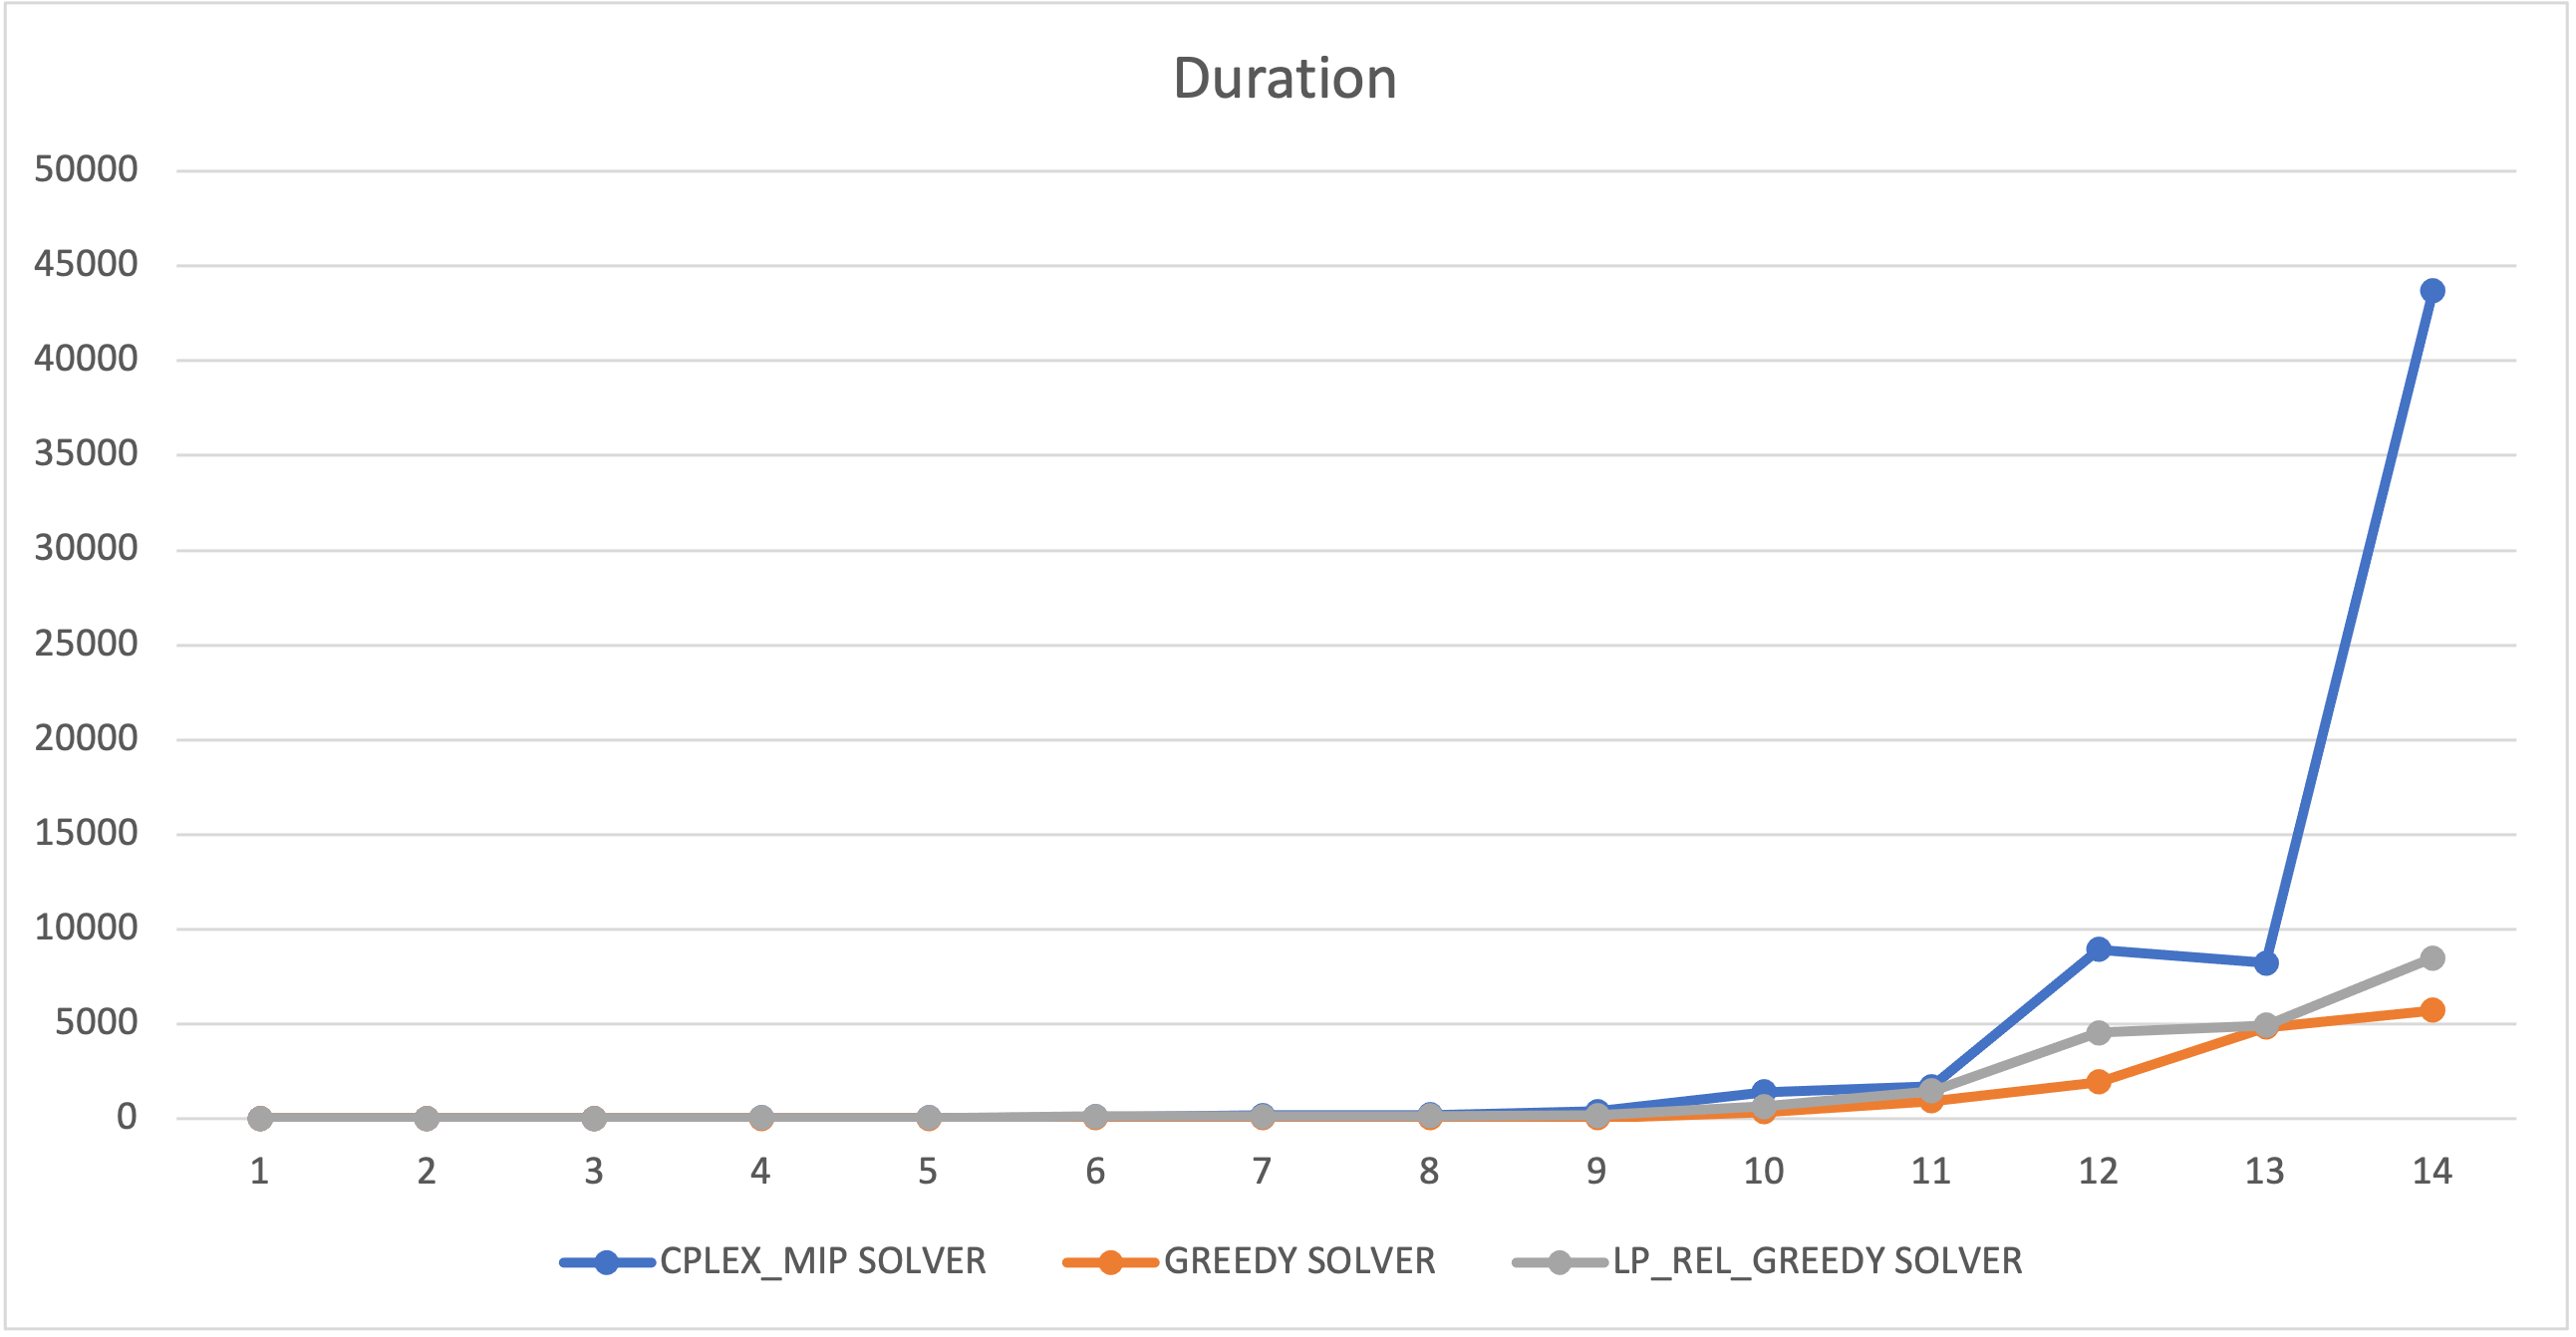
\includegraphics[width=12cm]{durations_no_rh}
            \caption{Durations-No Rolling Horizon Constraints}
            \label{fig:fig_durations_no_rh}
        \end{figure}

        \begin{table}[htb]
                \centering
                \caption[Short Caption for LoT]{\% Objective Value Differentiation-No Rolling Horizon Constraints}\label{table:tbl_test_obj_diff_no_rh}
            \csvautobooktabular{test_results_objective_diff_no_rh.csv}
        \end{table}
        \begin{figure}[htp]
            \centering
            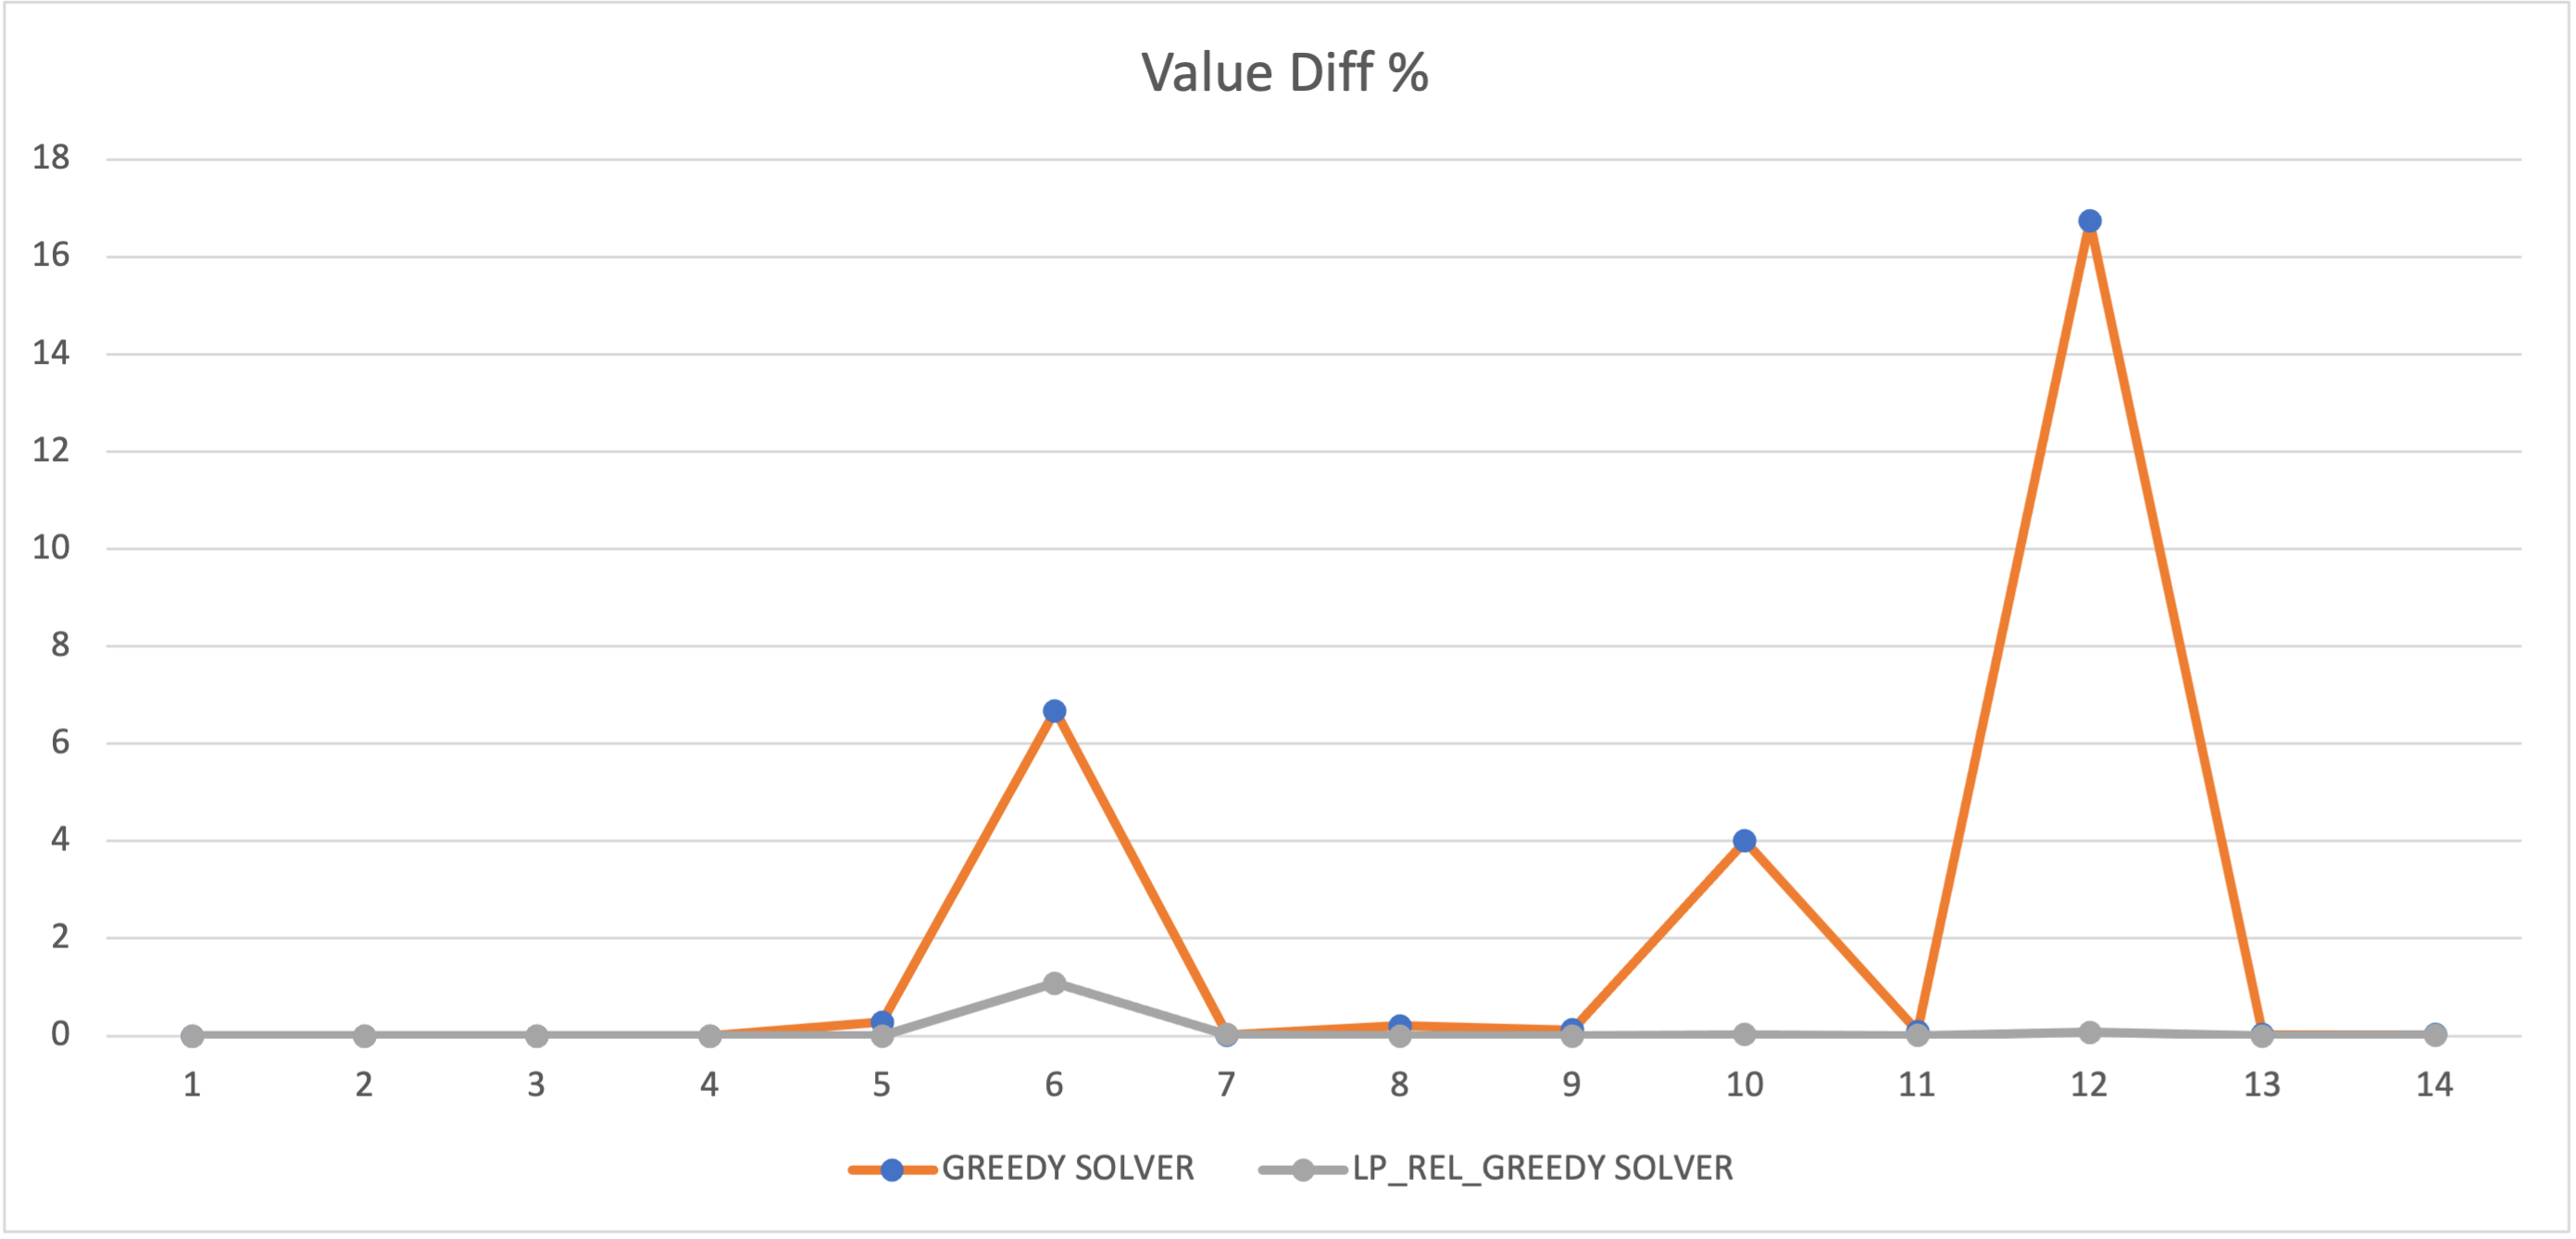
\includegraphics[width=12cm]{value_diff_no_rh}
            \caption{\% Objective Value Differentiation-No Rolling Horizon Constraints}
            \label{fig:fig_value_diff_no_rh}
        \end{figure}

        \begin{table}[htb]
                \centering
                \caption[Short Caption for LoT]{Durations at Phase-1 With Rolling Horizon Constraints}\label{table:tbl_test_durations_with_rh_ph1}
            \csvautobooktabular{test_results_durations_with_rh_ph1.csv}
        \end{table}
        \begin{table}[htb]
                \centering
                \caption[Short Caption for LoT]{Durations at Phase-2 With Rolling Horizon Constraints}\label{table:tbl_test_durations_with_rh_ph2}
            \csvautobooktabular{test_results_durations_with_rh_ph2.csv}
        \end{table}
        \begin{table}[htb]
                \centering
                \caption[Short Caption for LoT]{\% Objective Value Differentiation at Phase-2 with Rolling Horizon Constraints}\label{table:tbl_test_obj_diff_with_rh_ph1}
            \csvautobooktabular{test_results_objective_diff_with_rh_ph1.csv}
        \end{table}
        \begin{table}[htb]
                \centering
                \caption[Short Caption for LoT]{\% Objective Value Differentiation at Phase-2 with Rolling Horizon Constraints}\label{table:tbl_test_obj_diff_with_rh_ph2}
            \csvautobooktabular{test_results_objective_diff_with_rh_ph2.csv}
        \end{table}
\newpage
        \begin{figure}[htp]
            \centering
            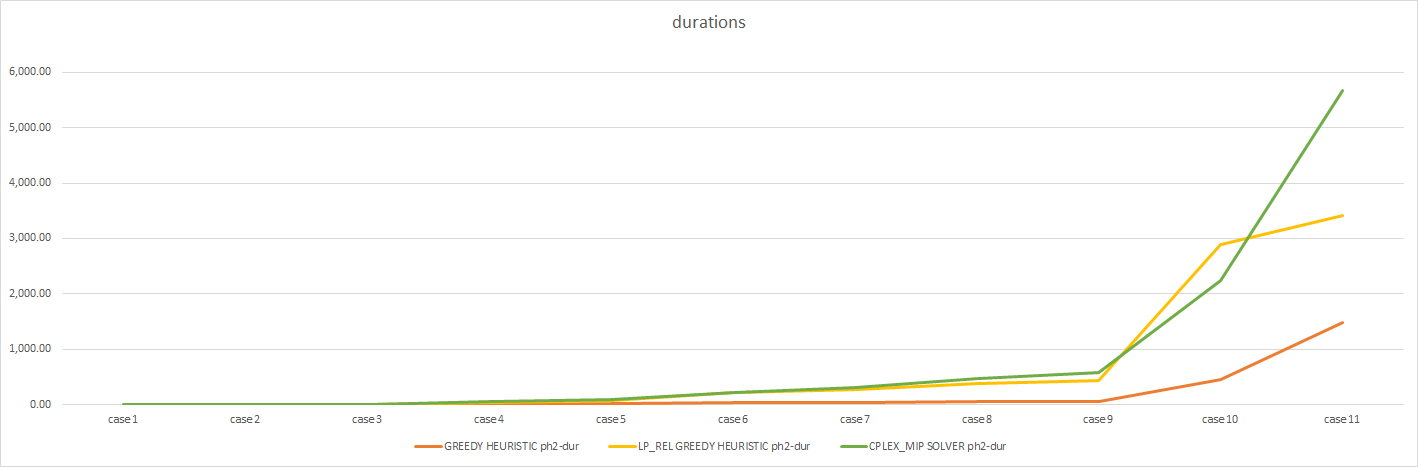
\includegraphics[width=20cm]{durations_with_rh}
            \caption{Durations with Rolling Horizon Constraints}
            \label{fig:fig_durations_with_rh}
        \end{figure}

        \begin{figure}[htp]
            \centering
            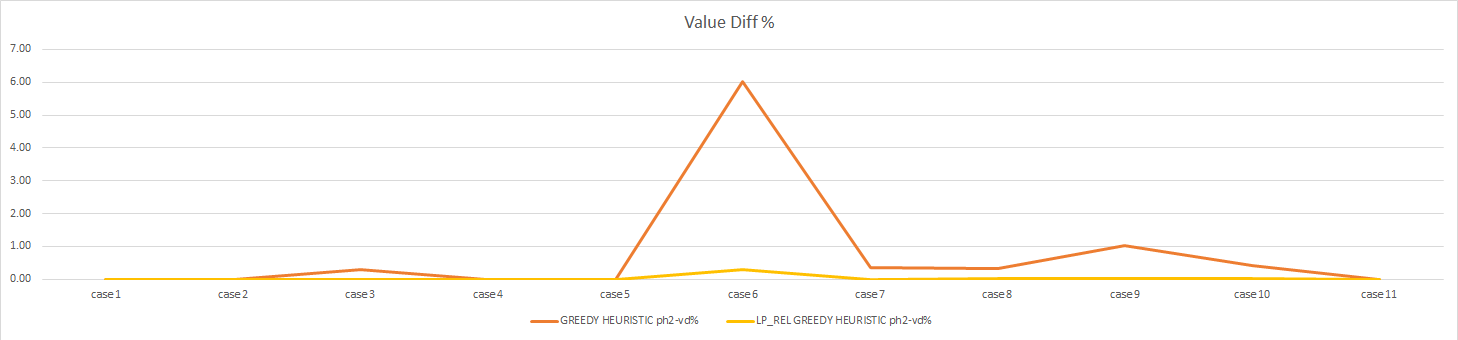
\includegraphics[width=20cm]{value_diff_with_rh}
            \caption{\% Objective Value Differentiation}
            \label{fig:fig_durations_with_rh}
        \end{figure}
    \end{landscape}
    \clearpage% Flush page
}

%%%%%%%%%%%%%%%%%%%%%%%%%%%%%%%%%%%%%%%%%%%%%%%%%%%%%%%%%%
%%%%%%%%%%%%%%%%%%%%%%%%%%%%%%%%%%%%%%%%%%%%%%%%%%%%%%%%%%

\newpage

\section{Conclusion} \label{s:conclusion}

%In this study, we focus on planning post-disaster infrastructure repair operations by considering interdependencies among different infrastructure networks. Since the functionality of a network component may affect the functionality of other components in the same or different networks, it is important to prioritize repairing critical damaged network components whose functionality may have significant effects on recovery times. We define a new post-disaster network recovery problem, which addresses coordinated routing of repair teams that visit the sites with damaged network components in multiple infrastructures to minimize total recovery times. We present a mathematical model and a practical simulated annealing heuristic to determine the order of repairs for each team. To test the proposed methods, we present a computational study by focusing on a setting with two interdependent infrastructure networks, such as power and gas. 


%{\color{blue} This study contributes to the literature in three main ways. First, we introduce a new coordinated post-disaster repair routing problem that incorporates functional interdependencies among multiple lifeline infrastructures. We show that ignoring such interdependencies can cause significant delays in infrastructure recovery times, which may affect survival and well-being of affected people. Secondly, we develop a novel mathematical model, which supports effective prioritization of repairing damaged network components by simultaneously considering infrastructure interdependencies, network travel times, component repair times, as well as the importance of components, which may represent the number of people that can be served once a node starts functioning or the criticality of services provided (e.g., providing electricity to the hospitals). Finally, given the limitations of the mathematical model to solve large size problem instances, we present an efficient simulated annealing metaheuristic that can find high quality solutions for realistic size instances in reasonable times. We design and test intensification and diversification strategies to improve the solution performance of the proposed algorithm.  Our computational results suggest that our metaheuristic, which incorporates an optimization model to address complexities brought by the interdependency structure in our problem, can solve a variety of instances with different characteristics effectively and support making coordinated repair planning after a disaster. In summary, our study makes a theoretical contribution to both disaster management and synchronized vehicle routing literature by defining a new coordinated routing problem that addresses interdependencies among infrastructure networks and a methodological contribution by formulating and solving a difficult optimization problem effectively. Our findings can also facilitate the coordination of post-disaster infrastructure repair efforts in practice.}

%Future research can focus on developing alternative solution methods for the proposed coordinated repair routing problem. Moreover, while the proposed problem assumes identical repair teams, in reality, the size and capabilities of repair teams may be different. Future research can extend the proposed problem by incorporating decisions related to developing repair plans in a setting where repair times of damaged components are affected by the size and capabilities of the repair teams.

\newpage

\bibliographystyle{chicago}
\bibliography{references}

\end{document}